%!TEX root = ../EmbSW1.tex
\section{Event Based Systems}
\subsection{Reaktive Systeme}
Ein Reaktives System befindet sich in ständiger Interaktion mit der Umgebung, wobei die Umgebung dominiert und das System sich dieser unterordnet.
\begin{itemize}
	\item Viele Embedded Systems sind auch reaktive Systeme
	\item Reaktive Systeme reagieren auf (oft externe) Ereignisse
	\begin{itemize}
	\item Digitale Inputs
	\item Erreichen von analogen Schwellwerten
	\item Timer
	\item Buttonclicks und ähnliches in GUI
	\item etc.
	\end{itemize}
	\item Häufig bestehen auch Echtzeitanforerungen an reaktive Systeme
\end{itemize}

\subsection{Umsetzung von Ereignissen}
\begin{itemize}
	\item Ereignisse sind per Definition asynchron
	\item Ein "'normales"' Programm ist immer synchron (zuerst das, dann das, dann...)
	\item Ereignisse können von synchronen Programmen durch Polling verarbeitet werden
	\begin{itemize}
		\item[+] einfach zu implementieren
		\item sehr viele Leerabfragen $\rightarrow$ unnötige Prozessorbelastung
		\item[$\bullet$] Leerabfragen können durch periodische Abfragen (Kopplung an Timer) reduziert aber nicht vermieden werden.
		\item[$\bullet$] Die maximale Reaktionszeit wird durch die Abfrageperiode und die Anzahl Abfragen definiert
	\end{itemize}
	\item Interrupt
	\begin{itemize}
		\item Non-vectored Interrupt (zentral)
		\begin{itemize}
			\item Alle Interrupts verzweigen zu einer gemeinsamen Adresse. Dort wird die Ursache bestimmt und zu einer spezifischen Behandlungsroutine verzweigt.
		\end{itemize}
		\item Vectored Interrupt (spezifisch)
		\begin{itemize}
			\item In einer Tabelle (Interruptvektortabelle) wird gespeichert, wohin bei welchem Interruptvektor verzweigt werden muss.
		\end{itemize}
	\end{itemize}
	\item	Interruptvektortabelle (IVT)
	\begin{itemize}
		\item Für jeden Vektor muss eingetragen werden, welches die Anfangsadresse der Interrupt Service Routine (ISR) ist, d.h. die IVT ist nichts anderes als eine Tabelle (Array) von Funktionspointern.
	\end{itemize}
\end{itemize}

\subsection{Model View Controller (MVC) aka Observer Pattern}
\begin{multicols}{2}
	\begin{itemize}
		\item Beim MVC wirkt das Model als Server, die Views sind Clients
		\item Jeder Client meldet beim Server an, welche Ereignisse ihn interessieren
		\item Diese Anmeldung, bzw. Registrierung erfolgt über eine Funktion, welche der Server anbietet:
		\begin{lstlisting}[style=C]
int foo_registerCb(foo_Event e, foo_cbFunction f);
// registers function 'f' on event 'e'
// sometimes called attach()
		\end{lstlisting}
		\item Der Server trägt diesen Funktionspointer f in eine Tabelle ein und ruft bei Eintreten des Ereignisses alle registrierten Funktionen der Reihe nach je über den eingetragenen Funktionspointer auf
	\end{itemize}
\columnbreak
	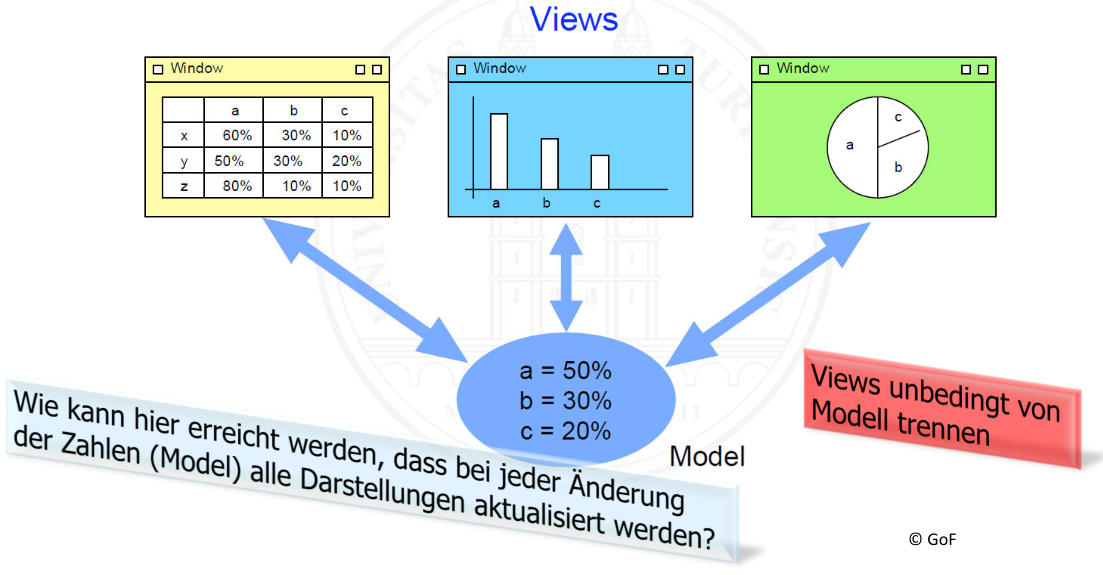
\includegraphics[width=\linewidth]{images/EventBasedSystems/MVC}
\end{multicols}

\subsubsection{Umsetzung der Callback-Funktionen in C}
\begin{itemize}
	\item Funktionspointer \lstinline[style=C]{foo_cbFunction} zu Callback-Funktionen definieren\\
	Annahme: Callback-Funktionen haben die Schnittstelle \lstinline[style=C]{void f(int);}
	\begin{lstlisting}[style=C]
typedef void (*foo_cbFunction)(int);
	\end{lstlisting}

	\item Tabelle von Funktionspointern für jeden Event definieren
	\begin{lstlisting}[style=C]
foo_cbFunction evClient[evNum] = {0};
	\end{lstlisting}

	\item Aufruf der registrierten Clientfunktionen beim Eintreten des Events
	\begin{lstlisting}[style=C]
for (i = 0; i < evNum; ++i)
{
  if (evClient[i] != 0) // entry found
  {
    evClient[i](arg);   // call client through function ptr
  }
}
	\end{lstlisting}
\end{itemize}

\subsubsection{Vorteile der Callback-Funktionen}
\begin{itemize}
	\item Die Views werden asynchron genau informiert, wenn sich etwas geändert hat im Model
	\item An und für sich sind alle registrierten Funktionen nichts anderes als Eventhandler eines bestimmten Events
	\item Dadurch wird die Darstellung (die Definition der registrierten Funktionen) sauber von den Daten (Model) entkoppelt
\end{itemize}
